%%%%%%%%%%%%%%%%%%%%%%%%%%%%% Define Article %%%%%%%%%%%%%%%%%%%%%%%%%%%%%%%%%%
\documentclass{article}
%%%%%%%%%%%%%%%%%%%%%%%%%%%%%%%%%%%%%%%%%%%%%%%%%%%%%%%%%%%%%%%%%%%%%%%%%%%%%%%

%%%%%%%%%%%%%%%%%%%%%%%%%%%%% Using Packages %%%%%%%%%%%%%%%%%%%%%%%%%%%%%%%%%%
\usepackage{geometry}
\usepackage{graphicx}
\usepackage{amssymb}
\usepackage{amsmath}
\usepackage{amsthm}
\usepackage{empheq}
\usepackage{mdframed}
\usepackage{booktabs}
\usepackage{lipsum}
\usepackage{graphicx}
\usepackage{color}
\usepackage{psfrag}
\usepackage{pgfplots}
\usepackage{bm}
\usepackage{enumitem}
\usepackage{hyperref}
\usepackage{multirow}
\usepackage{longtable}
%%%%%%%%%%%%%%%%%%%%%%%%%%%%%%%%%%%%%%%%%%%%%%%%%%%%%%%%%%%%%%%%%%%%%%%%%%%%%%%

% Other Settings

%%%%%%%%%%%%%%%%%%%%%%%%%% Page Setting %%%%%%%%%%%%%%%%%%%%%%%%%%%%%%%%%%%%%%%
\geometry{a4paper}

%%%%%%%%%%%%%%%%%%%%%%%%%% Define some useful colors %%%%%%%%%%%%%%%%%%%%%%%%%%
\definecolor{ocre}{RGB}{243,102,25}
\definecolor{mygray}{RGB}{243,243,244}
\definecolor{deepGreen}{RGB}{26,111,0}
\definecolor{shallowGreen}{RGB}{235,255,255}
\definecolor{deepBlue}{RGB}{61,124,222}
\definecolor{shallowBlue}{RGB}{235,249,255}
%%%%%%%%%%%%%%%%%%%%%%%%%%%%%%%%%%%%%%%%%%%%%%%%%%%%%%%%%%%%%%%%%%%%%%%%%%%%%%%

%%%%%%%%%%%%%%%%%%%%%%%%%% Define an orange box command %%%%%%%%%%%%%%%%%%%%%%%%
\newcommand\orangebox[1]{\fcolorbox{ocre}{mygray}{\hspace{1em}#1\hspace{1em}}}
%%%%%%%%%%%%%%%%%%%%%%%%%%%%%%%%%%%%%%%%%%%%%%%%%%%%%%%%%%%%%%%%%%%%%%%%%%%%%%%

%%%%%%%%%%%%%%%%%%%%%%%%%%%% English Environments %%%%%%%%%%%%%%%%%%%%%%%%%%%%%
\newtheoremstyle{mytheoremstyle}{3pt}{3pt}{\normalfont}{0cm}{\rmfamily\bfseries}{}{1em}{{\color{black}\thmname{#1}~\thmnumber{#2}}\thmnote{\,--\,#3}}
\newtheoremstyle{myproblemstyle}{3pt}{3pt}{\normalfont}{0cm}{\rmfamily\bfseries}{}{1em}{{\color{black}\thmname{#1}~\thmnumber{#2}}\thmnote{\,--\,#3}}
\theoremstyle{mytheoremstyle}
\newmdtheoremenv[linewidth=1pt,backgroundcolor=shallowGreen,linecolor=deepGreen,leftmargin=0pt,innerleftmargin=20pt,innerrightmargin=20pt,]{theorem}{Theorem}[section]
\theoremstyle{mytheoremstyle}
\newmdtheoremenv[linewidth=1pt,backgroundcolor=shallowBlue,linecolor=deepBlue,leftmargin=0pt,innerleftmargin=20pt,innerrightmargin=20pt,]{definition}{Definition}[section]
\theoremstyle{myproblemstyle}
\newmdtheoremenv[linecolor=black,leftmargin=0pt,innerleftmargin=10pt,innerrightmargin=10pt,]{problem}{Problem}[section]
%%%%%%%%%%%%%%%%%%%%%%%%%%%%%%%%%%%%%%%%%%%%%%%%%%%%%%%%%%%%%%%%%%%%%%%%%%%%%%%

%%%%%%%%%%%%%%%%%%%%%%%%%%%%%%% Plotting Settings %%%%%%%%%%%%%%%%%%%%%%%%%%%%%
\usepgfplotslibrary{colorbrewer}
\pgfplotsset{width=8cm,compat=1.9}
% \graphicspath{./imgs/}
%%%%%%%%%%%%%%%%%%%%%%%%%%%%%%%%%%%%%%%%%%%%%%%%%%%%%%%%%%%%%%%%%%%%%%%%%%%%%%%

%%%%%%%%%%%%%%%%%%%%%%%%%%%%%%% Title & Author %%%%%%%%%%%%%%%%%%%%%%%%%%%%%%%%
\title{Tarea 5 - RDF y SVM}
\author{Leonel Guerrero \\ Carnet: 1810638}
%%%%%%%%%%%%%%%%%%%%%%%%%%%%%%%%%%%%%%%%%%%%%%%%%%%%%%%%%%%%%%%%%%%%%%%%%%%%%%%

\begin{document}
\maketitle

\section*{Pregunta 1}

\subsection*{Enunciado}
En la demostración realizada en clase de que la función de base radial $k(x, z) = \text{exp}\left\{ \frac{-||x-z||^2}{\sigma^2} \right\}$ es un kernel se usaron varias propiedades. Demuestre cada una de las propiedades usadas para llegar a ese resultado.

\subsection*{Solución}

Las propiedades que se usaron para demostrar que $k(x, z) = \text{exp}\left\{ \frac{-||x-z||^2}{\sigma^2} \right\}$ es un kernel son las siguientes:

\begin{itemize}
  \item $k(x, z) = ck_1(x, z) \quad \forall c \in \mathbb{R^+} \land x, z \in \mathbb{R}^n$
  \item $k(x, z) = f(x)k_1(x, z)f(z) \quad f: \mathbb{R}^n \rightarrow \mathbb{R}$
  \item $k(x, z) = \text{exp}(k_1(x, z))$
\end{itemize}

Demostremos cada una de estas propiedades, para cada una de ellas, se usará la  definición de kernel:

\begin{equation*}
  k(x, z) = \phi(x)^t\phi(z) \quad \forall x, z \in \mathbb{R}^n
\end{equation*}

Es decir, que la función $k(x, z)$ es un kernel si se puede expresar como el producto de dos funciones.

\subsubsection*{Propiedad 1}

\begin{proof} Por la definición de kernel se tiene:
  \begin{align*}
    ck_1(x, z)          & = c\phi_1(x)^t\phi_1(z) \qquad \qquad \quad \text{Transformando $c$ convenientemente y sabiendo que $c\in \mathbb{R}^+$} \\
                        & = \sqrt{c}\sqrt{c} \phi_1(x)^t\phi_1(z) \qquad \quad \text{Reordenando los términos }                                    \\
                        & = (\sqrt{c}\phi_1(x)^t) (\sqrt{c}\phi_1(z)) \quad \text{ Definiendo } \phi(x) = \sqrt{c}\phi_1(x)                        \\
                        & = \phi(x)^t\phi(z)                                                                                                       \\
    \Rightarrow \phi(x) & = \sqrt{c}\phi_1(x)
  \end{align*}

  Por lo tanto, por la definición de kernel, $k(x, z) = ck_1(x, z)$ es un kernel.

\end{proof}

\subsubsection*{Propiedad 2}

\begin{proof} Por la definición de kernel se tiene:
  \begin{align*}
    f(x)k_1(x, z)f(z)   & = f(x)\phi_1(x)^t\phi_1(z)f(z) \qquad \quad \text{Reordenando los términos y sabiendo que $f:\mathbb{R}^n\rightarrow \mathbb{R}$} \\
                        & = [f(x)\phi_1(x)^t] [f(z)\phi_1(z)] \qquad \text{Definiendo } \phi(x) = f(x)\phi_1(x)                                             \\
                        & = \phi(x)^t\phi(z)                                                                                                                \\
    \Rightarrow \phi(x) & = f(x)\phi_1(x)
  \end{align*}

  Por lo tanto, por la definición de kernel, $k(x, z) = f(x)k_1(x, z)f(z)$ es un kernel.

\end{proof}

\subsubsection*{Propiedad 3}

\begin{proof} Por la definición de kernel se tiene:
  \begin{align*}
    \text{exp}(k_1(x, z)) & = \sum_{n=0}^\infty \frac{k_1(x, z)^n}{n!} \qquad \quad \text{Expandiendo la exponencial por series de Taylor} \\
                          & = 1 + k_1(x, z) + \frac{(k_1(x, z))^2}{2!} + \frac{(k_1(x, z))^3}{3!} + \cdots                                 \\
  \end{align*}

  En la expresión anterior se aplicara la propiedad demostrada previamente de $k(x,z) = ck_1(x,z)$, para cada término de la serie de Taylor, también se puede apreciar fácilmente que la constante $1$ es un kernel (ya que $\phi(x) = 1 \Rightarrow k(x,z) = 1\times 1$) y por ultimo se aplicara la propiedad de que la suma de kernels es un kernel, $k(x,z) = k_1(x,z) + k_2(x,z)$, obteniendo:

  \begin{align*}
    \text{exp}(k_1(x, z)) & = 1 + k_1(x, z) + \frac{(k_1(x, z))^2}{2!} + \frac{(k_1(x, z))^3}{3!} + \cdots \\
                          & = k_1(x,z) + k_2(x,z) + k_3(x,z) + \cdots                                      \\
                          & = k(x,z)
  \end{align*}



  Por lo tanto, $k(x, z) = \text{exp}(k_1(x, z))$ es un kernel.

\end{proof}

\section*{Pregunta 2}

\subsection*{Enunciado}

Para el conjunto de datos spectra100.csv cuya verdadera relación entrada-salida esta en SpectraReal.csv:

\begin{enumerate}[label=(\alph*)]
  \item Obtenga un aproximador universal usando como base las funciones de base radial. Comente sobre los resultados de generalización conociendo la verdadera relación entrada-salida de los datos. En caso de presentar dificultades con el sistema resultante por sus dimensiones, elija 1 de cada 5 datos (muestreo) a lo largo del dominio y repita. Comente.
  \item Use regularización para el aproximador universal obtenido del apartado previo. Cual es el parámetro de regularización escogido. Argumente sus razones y muestre el trabajo parcial para llegar a su mejor modelo.
  \item Construya una red RBF para el mismo conjunto de datos. Cuales son los mejores paráme-\\tros de  su modelo, como ha sido la elección de los centros y los resultados en función de esa selección.
  \item Use un parámetro de regularización sobre su RBF resultado del apartado anterior. Cual es el parámetro de regularización que mejores resultados les da.

\end{enumerate}
Para esta pregunta usted puede usar cualquier tipo de entrenamiento (por métodos iterativos o resolviendo el sistema de interpolación) y deberá ser detallado en su informe de resultados. Anexe el código usado. Use métricas (error en datos de prueba, comparación contra curva real u otro) para justificar su elección

\subsection*{Respuesta}

\subsubsection*{Implementación Aproximador Universal y Red RBF}

\begin{itemize}
  \item Aproximador Universal
        \begin{itemize}
          \item \href{https://github.com/LeoGCode/Tarea-4--Backpropagation}{Github}
          \item \href{https://colab.research.google.com/drive/1c8swOFZ_sL5bQSOi91ajNDod2Arv-0x6?usp=sharing}{Google Colab}
        \end{itemize}

  \item Red RBF
        \begin{itemize}
          \item \href{https://github.com/LeoGCode/Tarea-4--Backpropagation}{Github}
          \item \href{https://colab.research.google.com/drive/1c8swOFZ_sL5bQSOi91ajNDod2Arv-0x6?usp=sharing}{Google Colab}
        \end{itemize}
\end{itemize}

\subsubsection*{Análisis de Resultados}
\begin{itemize}
  \item \textbf{Aproximador Universal sin Regularización}
        En el código hay una celda, debajo del titulo "Test the network" con los test realizados probando diferentes parámetros para el valor de c, es decir, el parámetro de fuerza sobre la interpolación, con tres diferentes kernels (multicuadratica, multicuadratica inversa y gaussiana)

        Los parámetros mas representativos se pueden ver en las siguientes gráficas

        \begin{figure}[!ht]
          \centering
          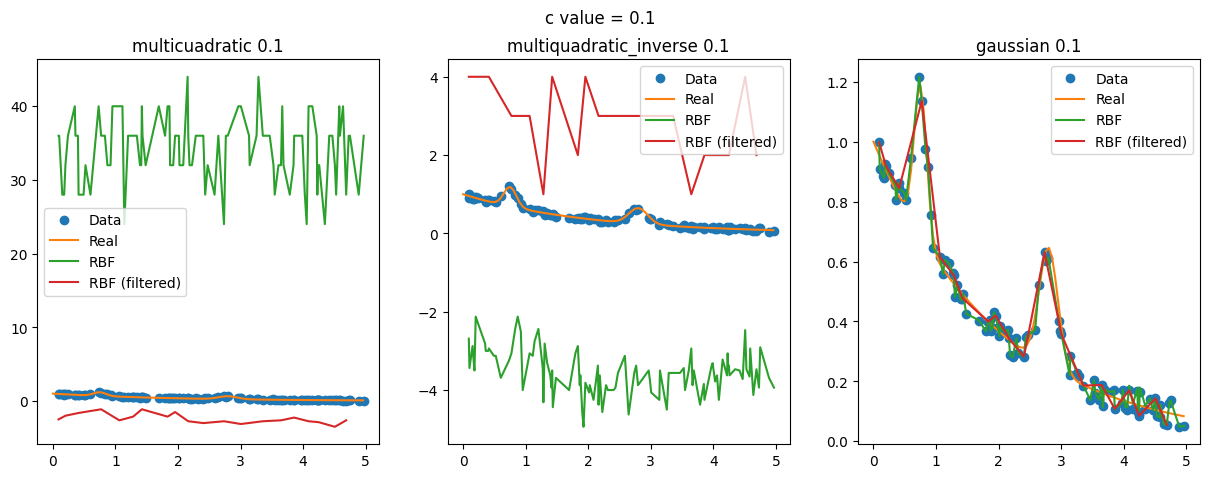
\includegraphics[width=1\textwidth]{./imgs/AU/au1.png}
          \caption{Aproximador Universal sin Regularización con $c=0.1$}
          \label{fig:1}
        \end{figure}

        \begin{figure}[!ht]
          \centering
          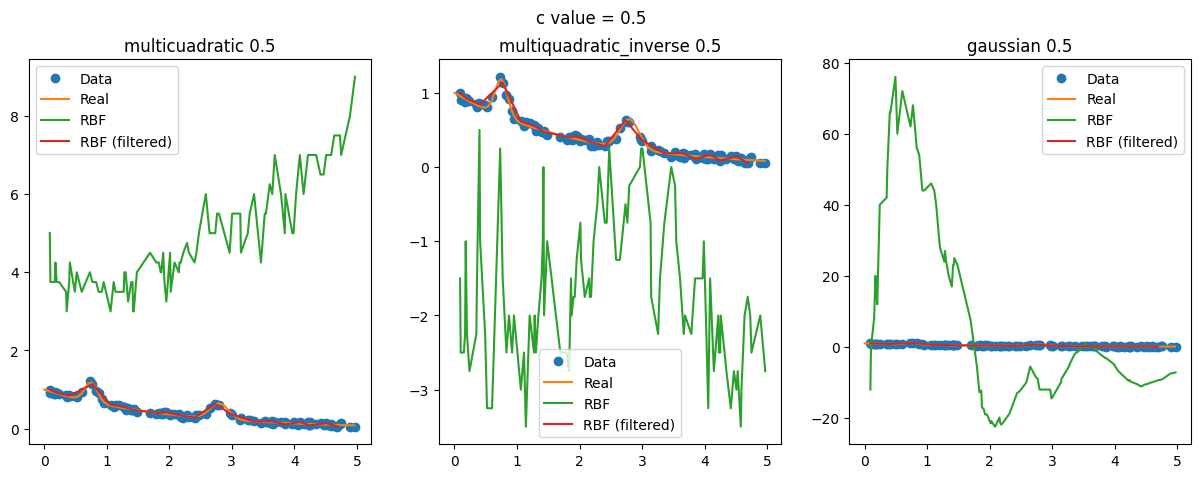
\includegraphics[width=1\textwidth]{./imgs/AU/au2.png}
          \caption{Aproximador Universal sin Regularización con $c=0.5$}
          \label{fig:2}
        \end{figure}

        \begin{figure}[!ht]
          \centering
          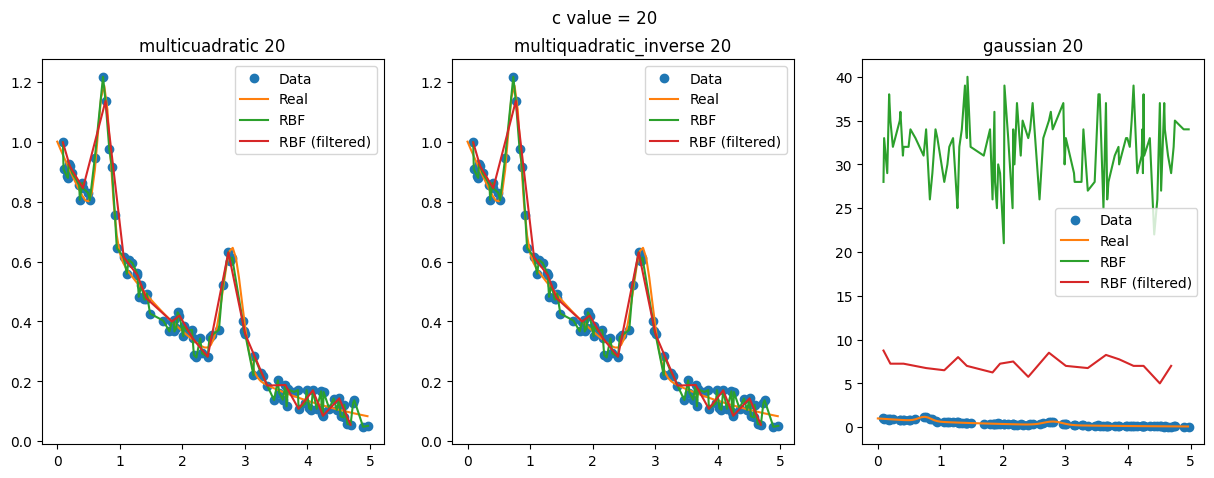
\includegraphics[width=1\textwidth]{./imgs/AU/au3.png}
          \caption{Aproximador Universal sin Regularización con $c=20$}
          \label{fig:3}
        \end{figure}

        Se puede apreciar que cuando se trabaja con el kernel gaussiano los mejores valores de $c$ suelen ser pequeños, mientras que con los otros dos kernels los mejores valores de c suelen ser grandes, esto se debe a que el kernel gaussiano es el que mejor se ajusta a los datos, por lo que se necesita una fuerza menor para que se ajuste a los datos, mientras que con los otros dos kernels se necesita una fuerza mayor para que se ajuste a los datos.

        También se puede apreciar que cuando no se escoge un valor de $c$ adecuado los pesos resultantes no se adaptan a los datos haciendo que se produzca una distorsión bastante grande en los resultados obtenidos como se puede apreciar en las multicuadraticas con $c=0.1$ y $c=0.5$ y en la gaussiana con $c=20$.

        Un hecho a destacar es el muestre realizado sobre los datos (tomando 1 de cada 5 puntos) en donde se puede apreciar que este muestre ayuda en ciertos casos a que los resultados mejores en la obtención de los pesos, esto se puede apreciar en las gráficas con el parámetro $c=0.5$ donde el resultado obtenido sin el muestro es distorsionado pero con el muestreo el resultado se ajusta a los valores reales.

  \item \textbf{Aproximador Universal con Regularización}
        En el código hay una celda, debajo del titulo "Test the network with Universal aproximator with regularization" con los test realizados probando diferentes parámetros para el valor de c (parámetro de forzamiento), con tres diferentes kernels (multicuadratica, multicuadratica inversa y gaussiana) y con diferentes valores de $\lambda$ para la regularización

        Los parámetros mas representativos se pueden ver en las siguientes gráficas

        \begin{figure}[!ht]
          \centering
          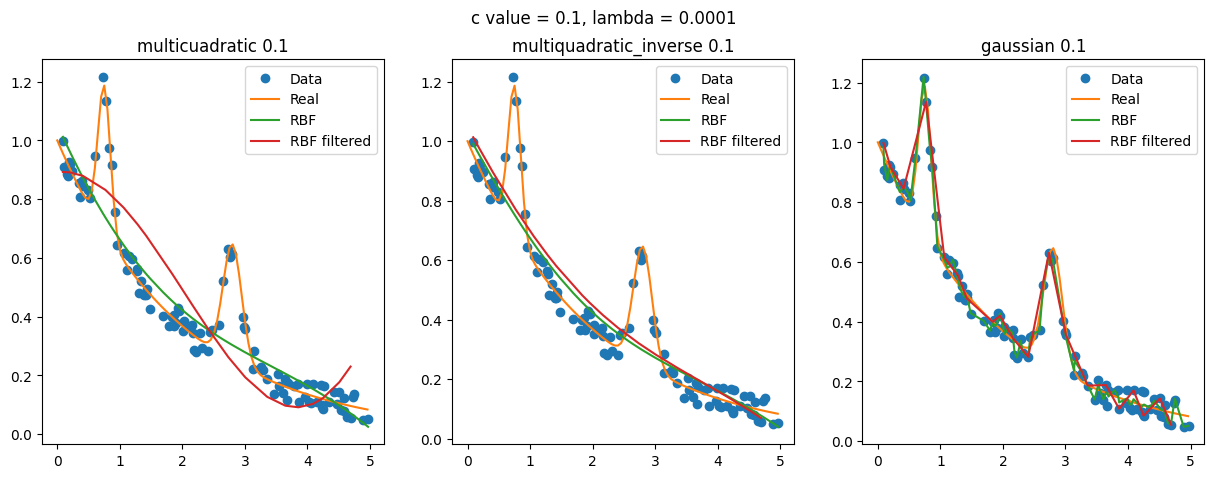
\includegraphics[width=1\textwidth, height=0.3\textwidth]{./imgs/AU/au_r1.png}
          \caption{Aproximador Universal con Regularización con $c=0.1$ y $\lambda=0.0001$}
          \label{fig:4}
        \end{figure}

        \begin{figure}[!ht]
          \centering
          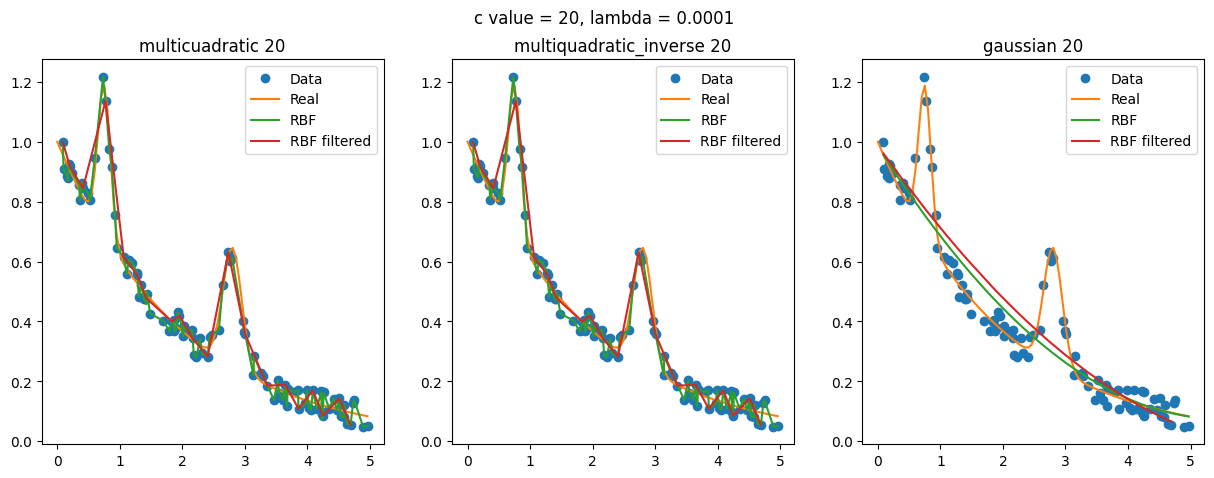
\includegraphics[width=1\textwidth, height=0.3\textwidth]{./imgs/AU/au_r2.png}
          \caption{Aproximador Universal con Regularización con $c=20$ y $\lambda=0.0001$}
          \label{fig:5}
        \end{figure}

        \begin{figure}[!ht]
          \centering
          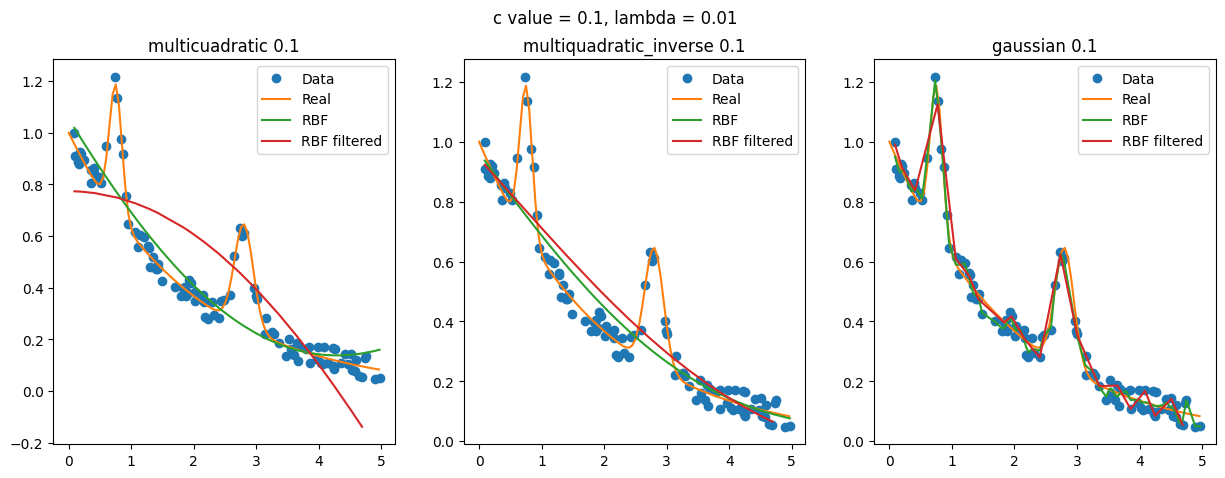
\includegraphics[width=1\textwidth, height=0.3\textwidth]{./imgs/AU/au_r3.png}
          \caption{Aproximador Universal con Regularización con $c=0.1$ y $\lambda=0.01$}
          \label{fig:6}
        \end{figure}

        Los mejores parámetros de las gráficas mostradas son la gaussiana con $c=0.1$ y $\lambda=0.0001$, en donde con estos parámetros se logra suavizar las  oscilaciones de la ultima parte de los datos y de la parte media de los datos, manteniendo la información de los picos con pocos datos.

        En las otras gráficas se puede apreciar que cuando el parámetro de $lambda$ es muy grande se logra suavizar los datos, pero se pierde la información de los picos con pocos datos, mientras que cuando el parámetro de $lambda$ es muy pequeño se logra mantener la información de los picos con pocos datos, pero se pierde la suavidad de los datos, sobre todo en la ultima parte de los datos.

  \item \textbf{RBF sin regularización}
        En el código hay una celda, debajo del titulo "Test the GRBF Network without regularization" con los test realizados probando diferentes parámetros del numero de centros $t$ y con diferentes valores de $\sigma$ para la función de activación gaussiana

        Los parámetros mas representativos se pueden ver en las siguientes gráficas

        \begin{figure}[!ht]
          \centering
          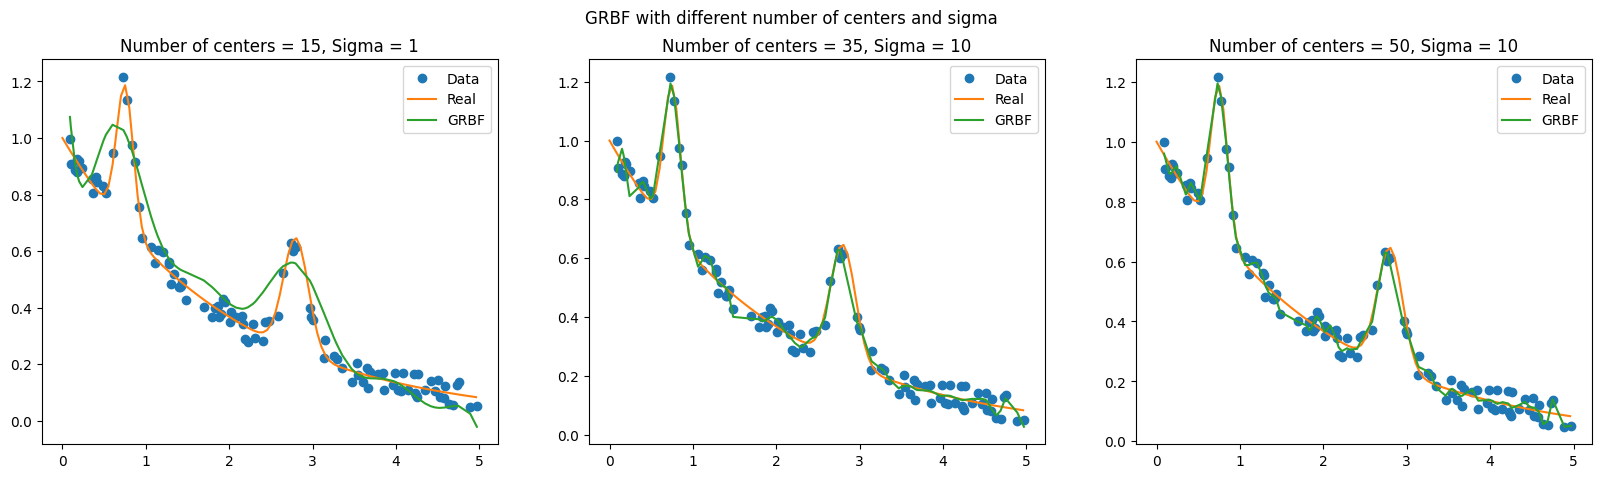
\includegraphics[width=1\textwidth]{./imgs/RBF/rbf.png}
          \caption{RBF sin Regularización}
          \label{fig:7}
        \end{figure}

        En estas gráficas se puede apreciar que se logra obtener un resultado bastante representativo de los datos sin muchas oscilaciones, en donde el mejore de los 3 gráficos tiene los parámetros $t=50$ y $\sigma=10$

  \item \textbf{RBF con regularización}
        En el código hay una celda, debajo del titulo "Test the GRBF Network with regularization" con los test realizados probando diferentes parámetros de regularización $\lambda$, estas pruebas se realizaron con los parámetros anteriormente mostrados ya que se considero que eran los mas representativos y con los cuales se podia obtener un mejor resultado de los datos.

        Los parámetros mas representativos se pueden ver en la gráfica a continuación

        \begin{figure}[!ht]
          \centering
          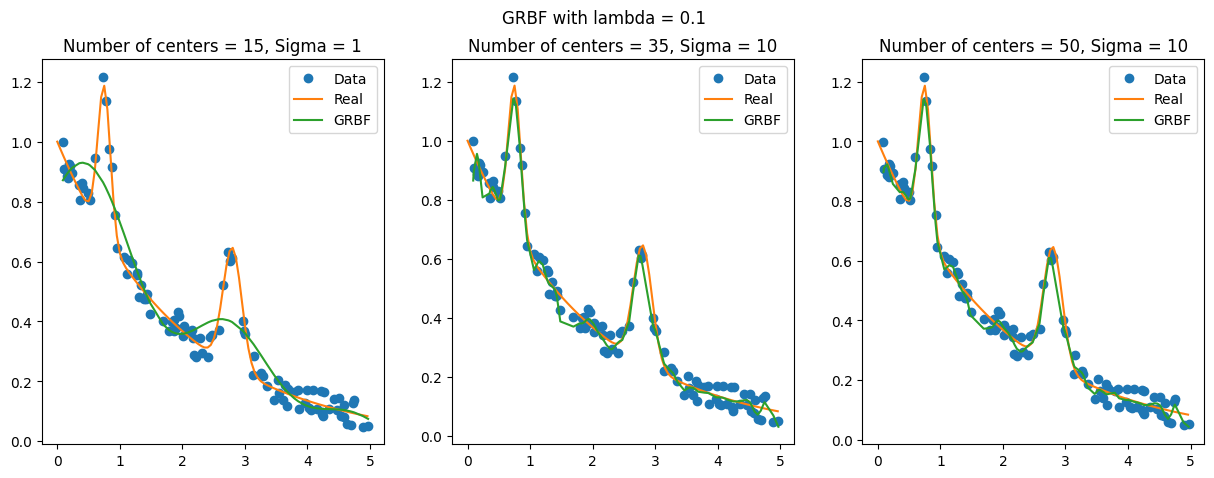
\includegraphics[width=1\textwidth]{./imgs/RBF/rbf_r.png}
          \caption{RBF con Regularización}
          \label{fig:8}
        \end{figure}

        En estas gráficas se puede apreciar que para el conjunto de datos dados, la regularización no aporta mucho a la obtención de los pesos, ya que se puede apreciar que los resultados obtenidos son muy similares a los obtenidos sin regularización, en donde el mejore de los 3 gráficos tiene los parámetros $t=50$, $\sigma=10$ y $\lambda=0.1$

\end{itemize}

\newpage
\section*{Pregunta 3}

\subsection*{Enunciado}

Para la siguiente pregunta usted puede elegir una implementación de una SVM tal que resuelva el problema planteado como:

\begin{equation*}
  \min J(w, w_0, \xi) = \frac{1}{2}||w||^2 + C\sum_{i=1}^N \xi_i
\end{equation*}

\[
  \text{Sujeto a: } \bigg\{
  \begin{array}{cc}
    d_i(w^tx + w_0) \geq 1 - \xi, & i = 1, 2, \dots, N \\
    \xi_i \geq 0,                 & i = 1, 2, \dots, N \\
  \end{array}
\]

Realice experimentos sobre el conjunto de datos provisto para los dos problemas de clasificación de textos variando el kernel (probar al menos dos kernels) y ajustando los parámetros del modelo lo mejor posible. ¿Cual fue la mejor maquina de aprendizaje obtenida? Indique el (los) criterio(s) usado para determinar su mejor modelo. La entrega constara de un pequeño informe con los resultados experimentales obtenidos comparando con los mejores resultados para la MLP de la tarea anterior y comentando sobre los resultados de generalización obtenidos y la escogería de sus parámetros. Anexe su código.

\subsection*{Resolución}

\subsubsection*{Implementación}

La implementación del SVM se hizo por medio de la librería de python scikit-learn\footnote{Scikit-learn: Machine Learning in Python, Pedregosa et al., JMLR 12, pp. 2825-2830, 2011. at \href{https://scikit-learn.org/stable/index.html}{home page} }, la cual tiene implementado el algoritmo de SVM con diferentes parámetros, el cual se puede utilizar para resolver el problema de clasificación de textos, para esto se utilizo la función SVC de la librería, la cual tiene como parámetros el kernel a utilizar, el valor de C y el valor de gamma, el cual es el parámetro del kernel gaussiano, el cual se utilizo para resolver el problema de clasificación de textos.

El código puede ser encontrado en:

\begin{itemize}
  \item \href{}{text}
  \item \href{}{text}
\end{itemize}

\subsubsection*{Análisis de resultados}

Se realizo una experimentación con la maquina de aprendizaje variando el kernel utilizado, el tratamiento de los datos (escalamiento por estandarización o normalización) y los dos parámetros libres del modelo, los cuales son el valor de C, el valor de gamma (o el grado del polinomio). Los kernel probados son el kernel lineal, el kernel gaussiano y el kernel polinomial, los valores de c y gamma probados fueron $[0.01, 0.1, 1, 10, 100]$ y los valores de grado del polinomio probados fueron $[2, 3, 4, 5, 6]$

A continuación se presenta una tabla con los valores mas representativos de la experimentación, tanto del conjunto de datos EarthSpace vs MedSci y LifeSci vs Agri, las tablas completas se puede encontrar en el repositorio en la carpeta "tables"

\begin{itemize}
  \item \textbf{EarthSpace vs MedSci}
\end{itemize}
% Please add the following required packages to your document preamble:
% \usepackage{multirow}
% \usepackage{longtable}
% Note: It may be necessary to compile the document several times to get a multi-page table to line up properly
\begin{longtable}{cccc|cccc|cc}
  \cline{2-10}
  \textbf{}                                                                            & \textbf{kernel}       & \multicolumn{2}{c|}{\textbf{linear}} & \multicolumn{4}{c|}{\textbf{rbf}} & \multicolumn{2}{c}{\textbf{poly}}                                                                                                    \\ \cline{2-10}
  \endfirsthead
  %
  \endhead
  %
  \textbf{}                                                                            & \textbf{gamma/degree} & \multicolumn{2}{c|}{\textbf{}}       & \multicolumn{2}{c}{\textbf{0.1}}  & \multicolumn{2}{c|}{\textbf{1}}   & \multicolumn{2}{c}{\textbf{4}}                                                                   \\ \cline{2-10}
  \textbf{}                                                                            & \textbf{train/test}   & \textbf{train}                       & \textbf{test}                     & \textbf{train}                    & \textbf{test}                  & \textbf{train} & \textbf{test} & \textbf{train} & \textbf{test} \\ \cline{2-10}
  \textbf{scaling}                                                                     & \textbf{c}            & \textbf{}                            & \textbf{}                         & \textbf{}                         & \textbf{}                      & \textbf{}      & \textbf{}     & \textbf{}      & \textbf{}     \\ \hline
  \multirow{3}{*}{\textbf{no scaling}}                                                 & \textbf{0.1}          & 0.77                                 & 0.74                              & 0.52                              & 0.64                           & 0.66           & 0.70          & 0.52           & 0.64          \\ \cline{7-8}
                                                                                       & \textbf{1}            & 0.82                                 & 0.75                              & 0.79                              & \multicolumn{1}{c|}{0.74}      & 0.93           & 0.76          & 1.00           & 0.72          \\ \cline{7-8}
                                                                                       & \textbf{10}           & 0.90                                 & 0.67                              & 0.87                              & 0.74                           & 1.00           & 0.73          & 1.00           & 0.74          \\ \hline
  \multirow{3}{*}{\textbf{\begin{tabular}[c]{@{}c@{}}standard\\ scaling\end{tabular}}} & \textbf{0.1}          & 0.98                                 & 0.63                              & 0.52                              & 0.64                           & 0.52           & 0.64          & 0.52           & 0.64          \\
                                                                                       & \textbf{1}            & 1.00                                 & 0.61                              & 1.00                              & 0.64                           & 1.00           & 0.64          & 1.00           & 0.68          \\
                                                                                       & \textbf{10}           & 1.00                                 & 0.61                              & 1.00                              & 0.64                           & 1.00           & 0.64          & 1.00           & 0.69          \\ \hline
  \multirow{3}{*}{\textbf{\begin{tabular}[c]{@{}c@{}}min-max\\ scaling\end{tabular}}}  & \textbf{0.1}          & 0.85                                 & 0.72                              & 0.52                              & 0.64                           & 0.52           & 0.64          & 1.00           & 0.70          \\
                                                                                       & \textbf{1}            & 0.95                                 & 0.65                              & 1.00                              & 0.75                           & 1.00           & 0.64          & 1.00           & 0.70          \\
                                                                                       & \textbf{10}           & 1.00                                 & 0.61                              & 1.00                              & 0.75                           & 1.00           & 0.64          & 1.00           & 0.70
\end{longtable}

\begin{itemize}
  \item \textbf{LifeSci vs Agri}
        \begin{longtable}{cccc|cc|cccc}
          \cline{2-10}
          \textbf{}                                                                            & \textbf{kernel}       & \multicolumn{2}{c|}{\textbf{linear}} & \multicolumn{2}{c|}{\textbf{rbf}} & \multicolumn{4}{c}{\textbf{poly}}                                                                                                                \\ \cline{2-10}
          \endfirsthead
          %
          \endhead
          %
          \textbf{}                                                                            & \textbf{gamma/degree} & \multicolumn{2}{c|}{\textbf{}}       & \multicolumn{2}{c|}{\textbf{1}}   & \multicolumn{2}{c}{\textbf{4}}    & \multicolumn{2}{c}{\textbf{5}}                                                                               \\ \cline{2-10}
          \textbf{}                                                                            & \textbf{train/test}   & \textbf{train}                       & \textbf{test}                     & \textbf{train}                    & \textbf{test}                  & \textbf{train} & \textbf{test}             & \textbf{train} & \textbf{test} \\ \cline{2-10}
          \textbf{scaling}                                                                     & \textbf{c}            & \textbf{}                            & \textbf{}                         & \textbf{}                         & \textbf{}                      & \textbf{}      & \textbf{}                 & \textbf{}      & \textbf{}     \\ \hline
          \multirow{3}{*}{\textbf{no scaling}}                                                 & \textbf{0.1}          & 0.66                                 & 0.64                              & 0.59                              & 0.55                           & 0.54           & 0.52                      & 1.00           & 0.63          \\ \cline{7-8}
                                                                                               & \textbf{1}            & 0.69                                 & 0.62                              & 0.88                              & 0.63                           & 1.00           & \multicolumn{1}{c|}{0.66} & 1.00           & 0.63          \\ \cline{7-8}
                                                                                               & \textbf{10}           & 0.72                                 & 0.62                              & 1.00                              & 0.61                           & 1.00           & 0.64                      & 1.00           & 0.63          \\ \hline
          \multirow{3}{*}{\textbf{\begin{tabular}[c]{@{}c@{}}standard\\ scaling\end{tabular}}} & \textbf{0.1}          & 0.74                                 & 0.61                              & 0.54                              & 0.52                           & 0.54           & 0.52                      & 0.54           & 0.52          \\
                                                                                               & \textbf{1}            & 0.74                                 & 0.60                              & 1.00                              & 0.52                           & 1.00           & 0.54                      & 1.00           & 0.53          \\
                                                                                               & \textbf{10}           & 0.74                                 & 0.59                              & 1.00                              & 0.52                           & 1.00           & 0.59                      & 1.00           & 0.55          \\ \hline
          \multirow{3}{*}{\textbf{\begin{tabular}[c]{@{}c@{}}min-max\\ scaling\end{tabular}}}  & \textbf{0.1}          & 0.70                                 & 0.62                              & 0.54                              & 0.52                           & 1.00           & 0.60                      & 1.00           & 0.60          \\
                                                                                               & \textbf{1}            & 0.73                                 & 0.61                              & 1.00                              & 0.52                           & 1.00           & 0.60                      & 1.00           & 0.60          \\
                                                                                               & \textbf{10}           & 0.74                                 & 0.60                              & 1.00                              & 0.52                           & 1.00           & 0.60                      & 1.00           & 0.60
        \end{longtable}
\end{itemize}

Como se puede apreciar en las tablas la mejor maquina de aprendizaje para el conjunto de datos EarthSpace vs MedSci es la SVM con kernel gaussiano (rbf), con un valor de $C = 1$ y un valor de $gamma = 1$, con una taza de aciertos de $0.93$ en el entrenamiento y $0.76$ en el conjunto de prueba (el mas alto  de todas las pruebas) mientras que para el conjunto de datos LifeSci vs Agri es la SVM con kernel polinomial, con un valor de $C = 1$ y un valor de $grado = 4$, con una taza de aciertos de $0.99$ en el entrenamiento y $0.65$ en el conjunto de prueba (el mas alto  de todas las pruebas)

Veamos la comparación de los resultados obtenidos con la MLP de la tarea anterior, en la siguiente tabla se puede apreciar los resultados obtenidos con la MLP y los resultados obtenidos con la SVM

\begin{longtable}{ccccc}
  \cline{2-5}
                                                                 & \multicolumn{2}{c}{SVM} & \multicolumn{2}{c}{MLP}                \\ \cline{2-5}
  \endfirsthead
  %
  \endhead
  %
                                                                 & train                   & test                    & train & test \\ \hline
  \begin{tabular}[c]{@{}c@{}}EarthSpace\\ vs MedSci\end{tabular} & 0.93                    & 0.76                    & 0.82  & 0.40 \\ \hline
  \begin{tabular}[c]{@{}c@{}}LifeSci\\ vs Agri\end{tabular}      & 1.00                    & 0.66                    & 0.63  & 0.46 \\ \hline
\end{longtable}
Como se puede apreciar en la tabla, la SVM obtuvo mejores resultados que la MLP, obteniendo mejores resultados tanto en el conjunto de entrenamiento como en el conjunto de prueba.

\end{document}